\section*{Appendix A}

\subsection*{A.1.1\ \ Numerikus stabilitás $dt = 10^{-3}$ év esetén}

{\centering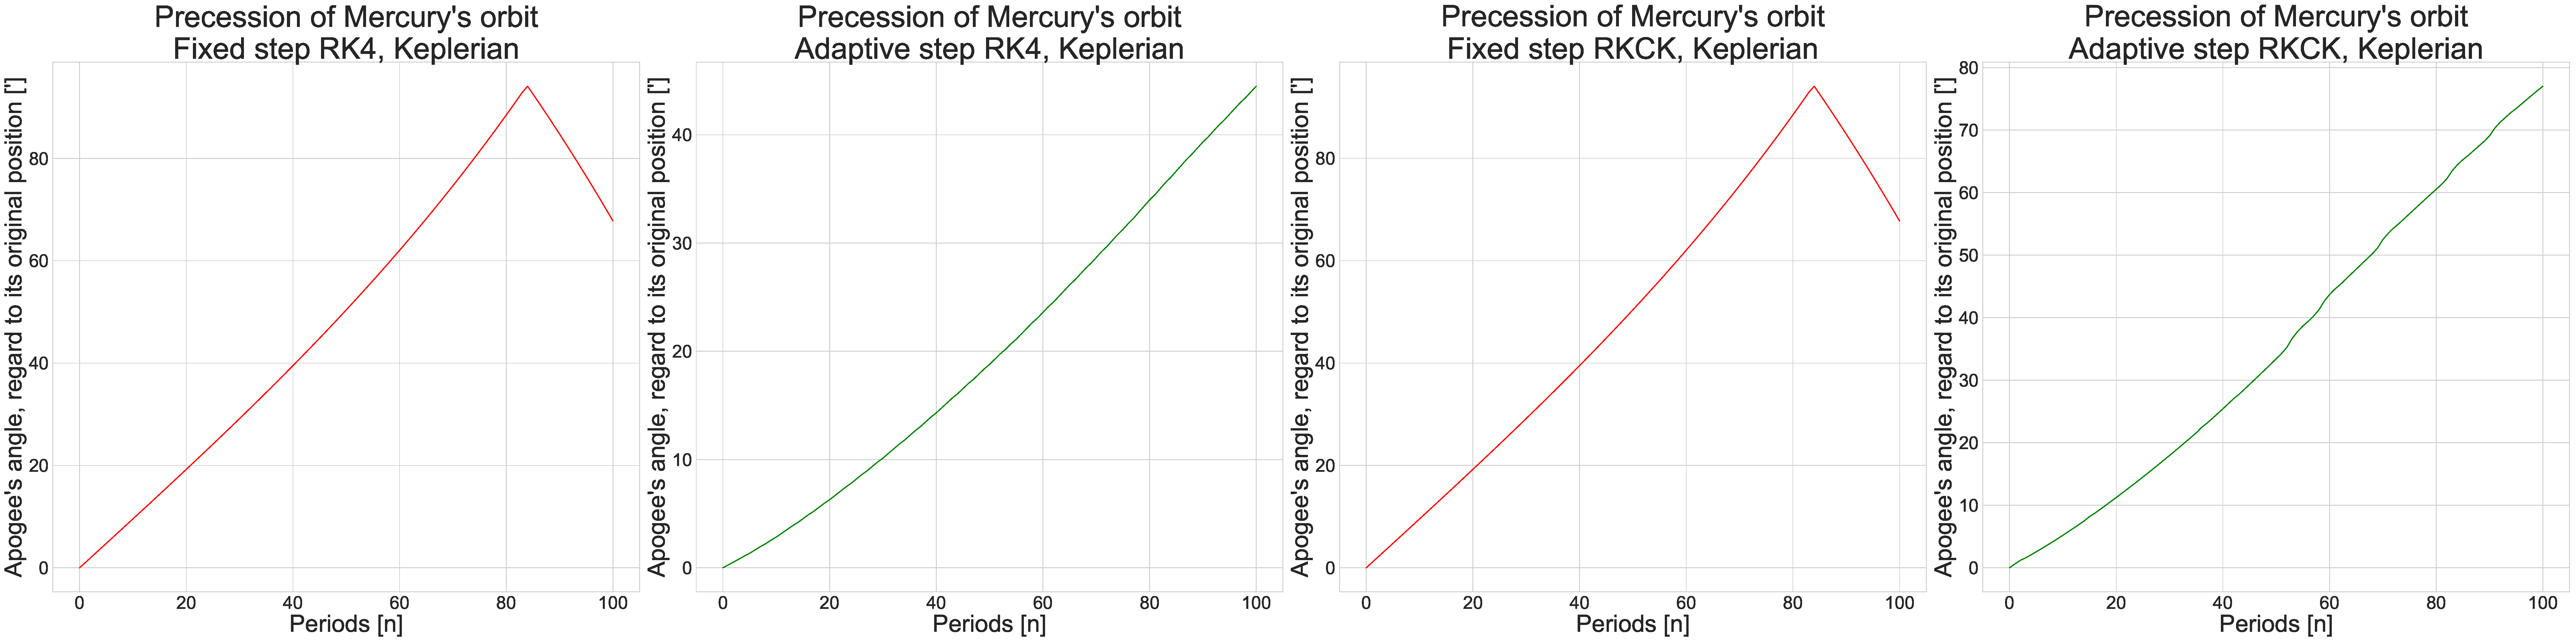
\includegraphics[width=\textwidth]{single_body/Mercury_precession_kepler_dt_1e-03_acc_1e-12.pdf}}
\captionof{figure}{Kepleri dinamika\\Lépésköz nagysága $0.001 = 10^{-3}$ év}\label{fig:1}
\hfill \break \break
{\centering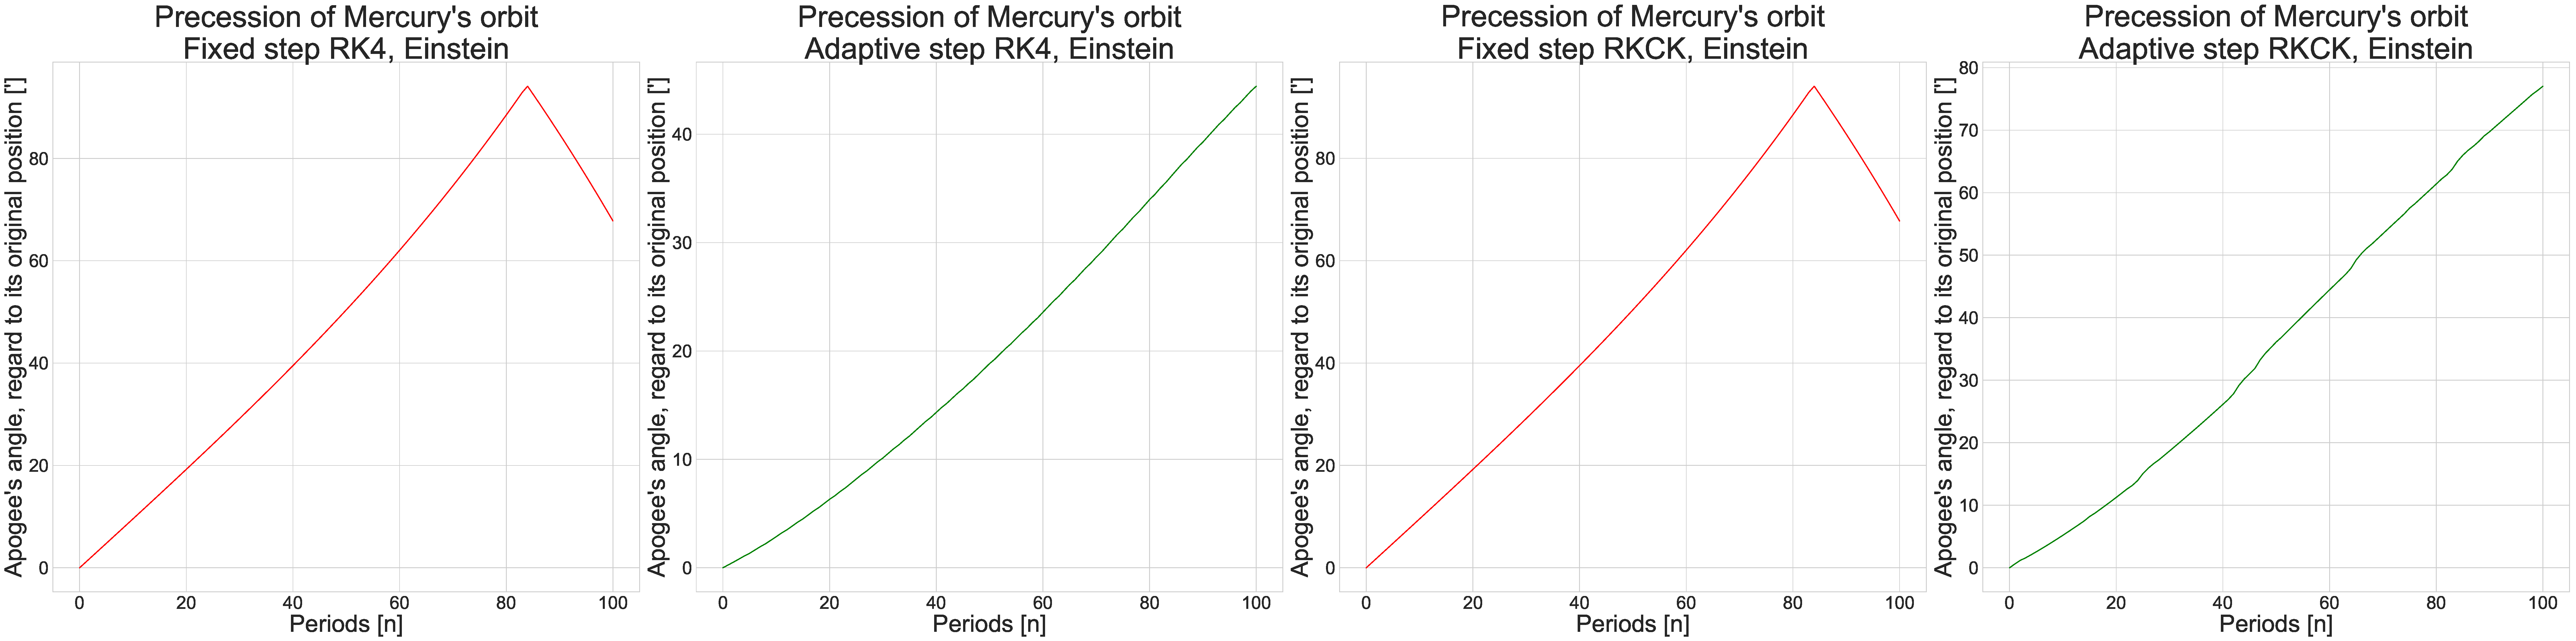
\includegraphics[width=\textwidth]{single_body/Mercury_precession_relat_dt_1e-03_acc_1e-12.pdf}}
\captionof{figure}{Relativisztikus dinamika\\Lépésköz nagysága $0.001 = 10^{-3}$ év}\label{fig:2}
\hfill \break \break
{\centering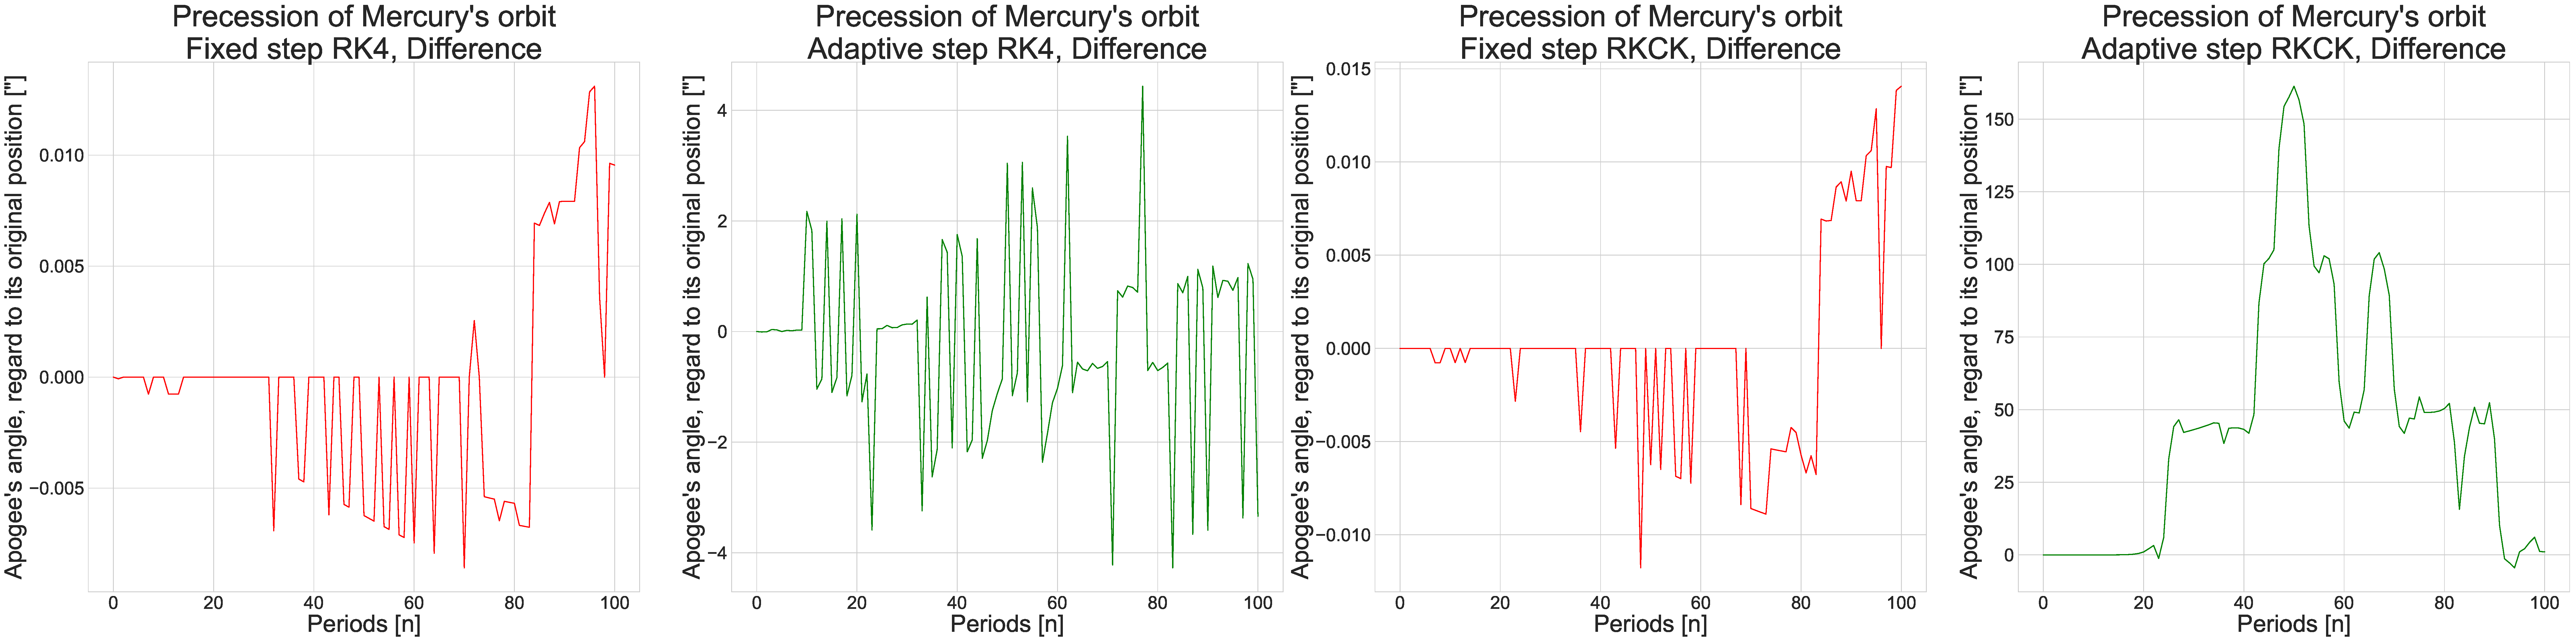
\includegraphics[width=\textwidth]{single_body/Mercury_precession_difference100_dt_1e-03_acc_1e-12.pdf}}
\captionof{figure}{A relativisztikus és a kepleri dinamika különbsége\\Lépésköz nagysága $0.001 = 10^{-3}$ év}\label{fig:3}

\newpage

\subsection*{A.1.2\ \ Numerikus stabilitás $dt = 10^{-4}$ év esetén}

{\centering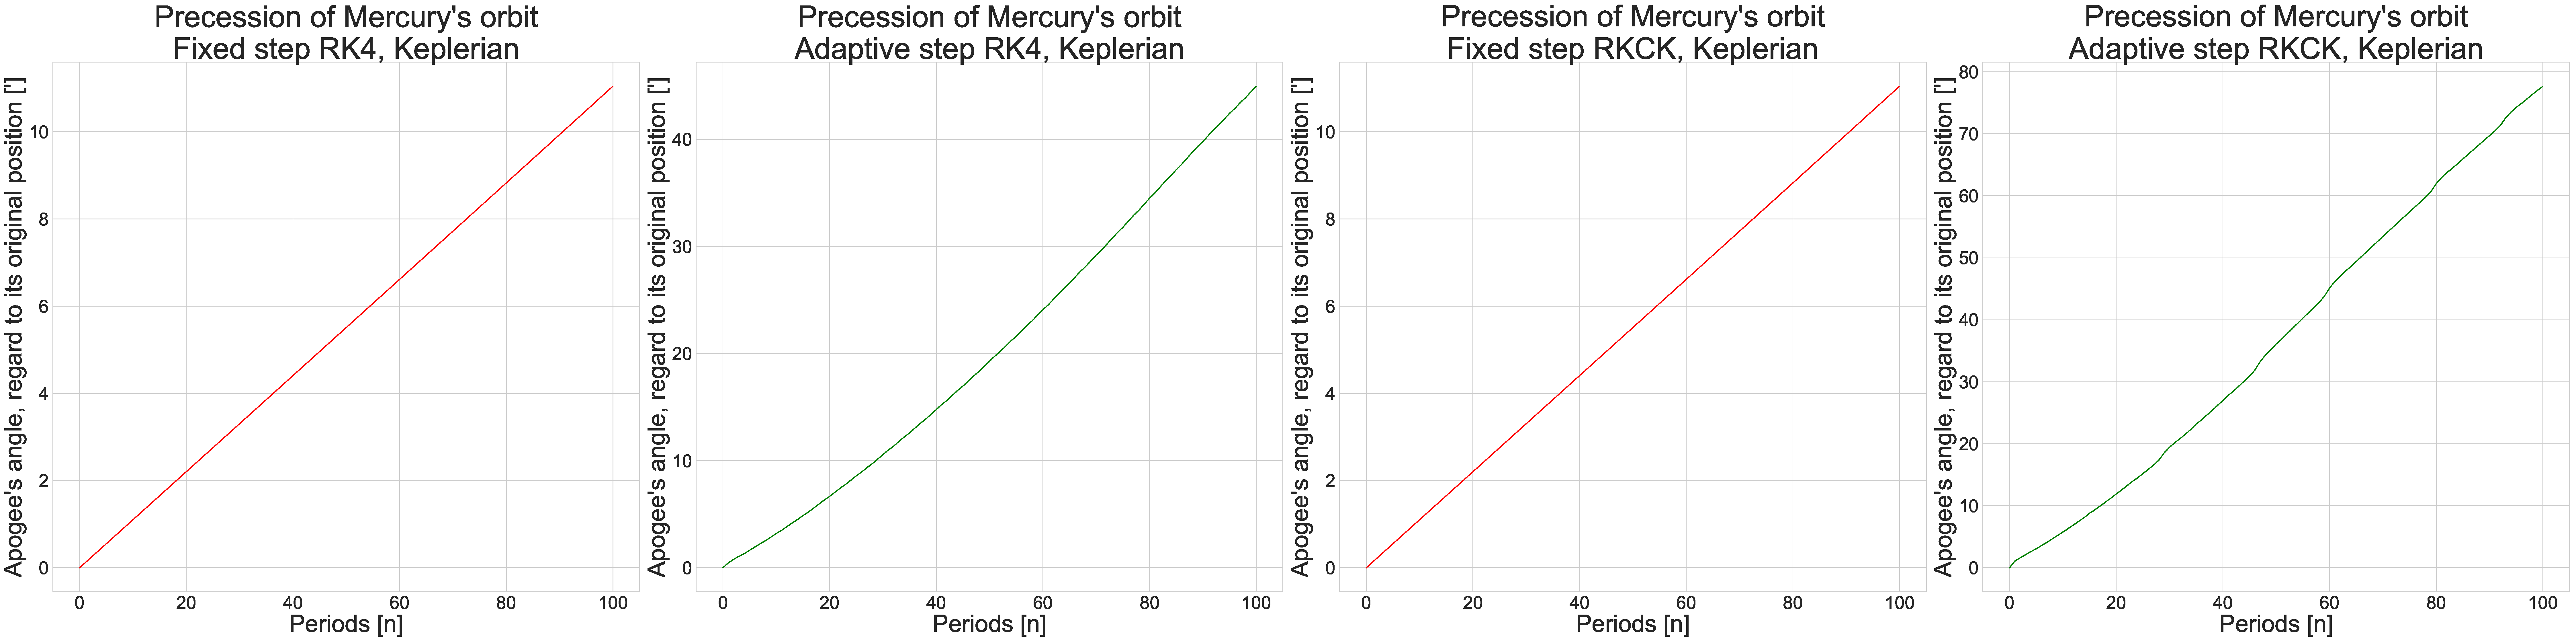
\includegraphics[width=\textwidth]{single_body/Mercury_precession_kepler_dt_1e-04_acc_1e-12.pdf}}
\captionof{figure}{Kepleri dinamika\\Lépésköz nagysága $0.0001 = 10^{-4}$ év}\label{fig:4}
\hfill \break \break
{\centering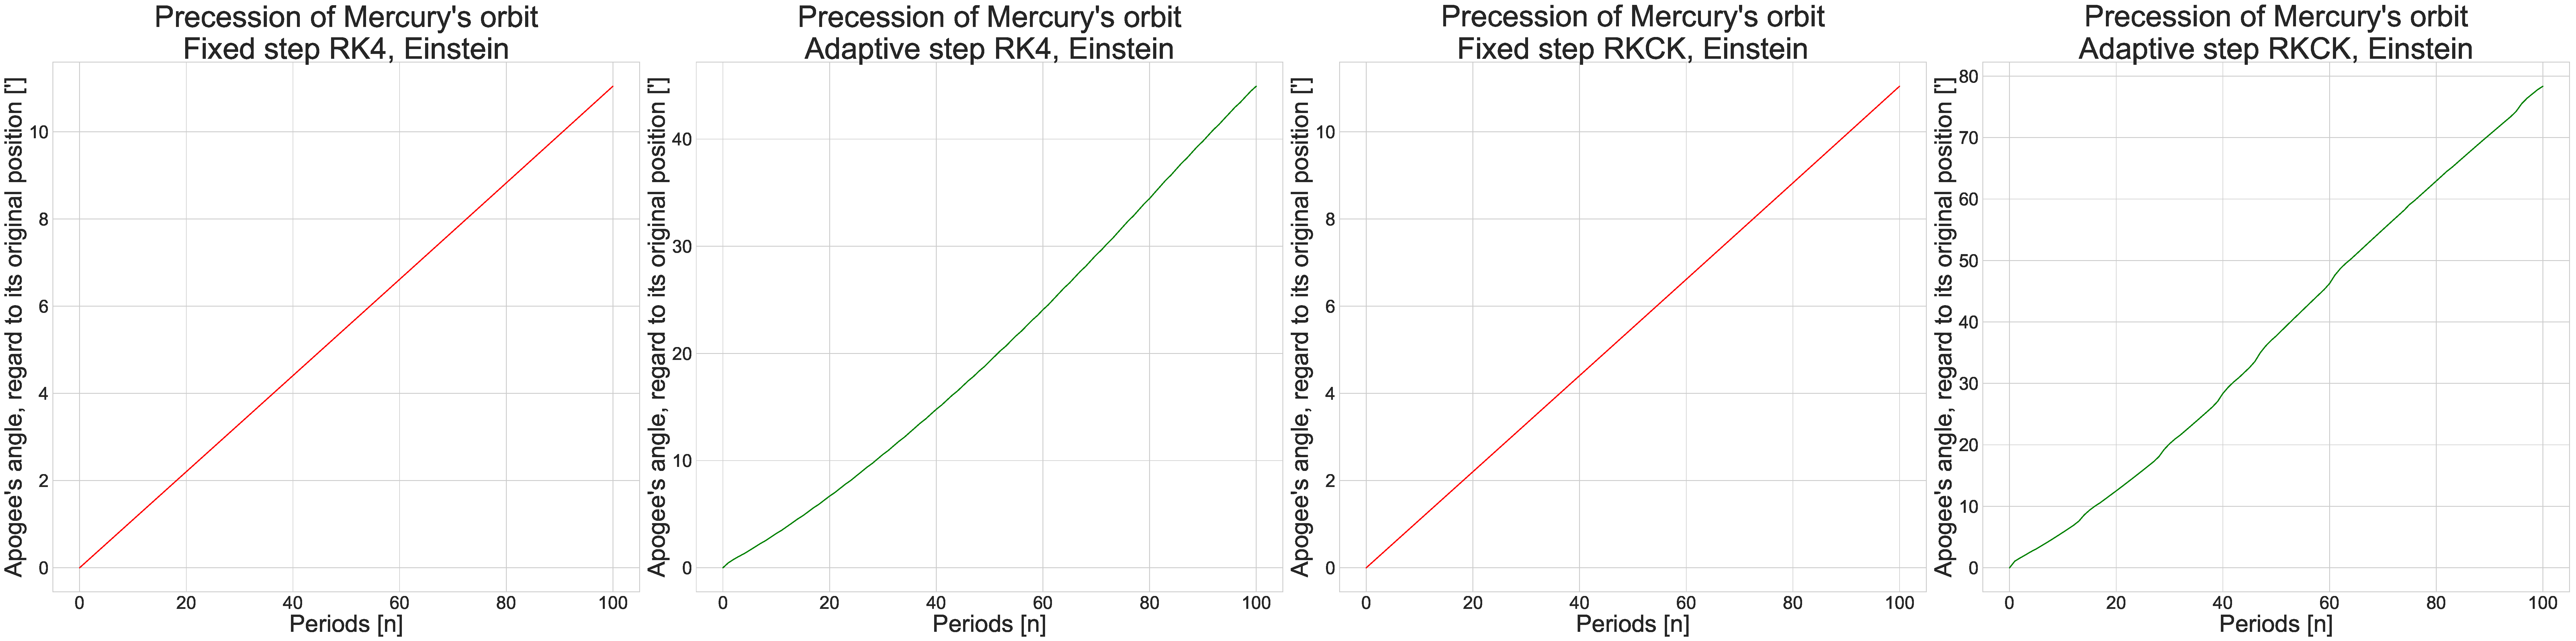
\includegraphics[width=\textwidth]{single_body/Mercury_precession_relat_dt_1e-04_acc_1e-12.pdf}}
\captionof{figure}{Relativisztikus dinamika\\Lépésköz nagysága $0.0001 = 10^{-4}$ év}\label{fig:5}
\hfill \break \break
{\centering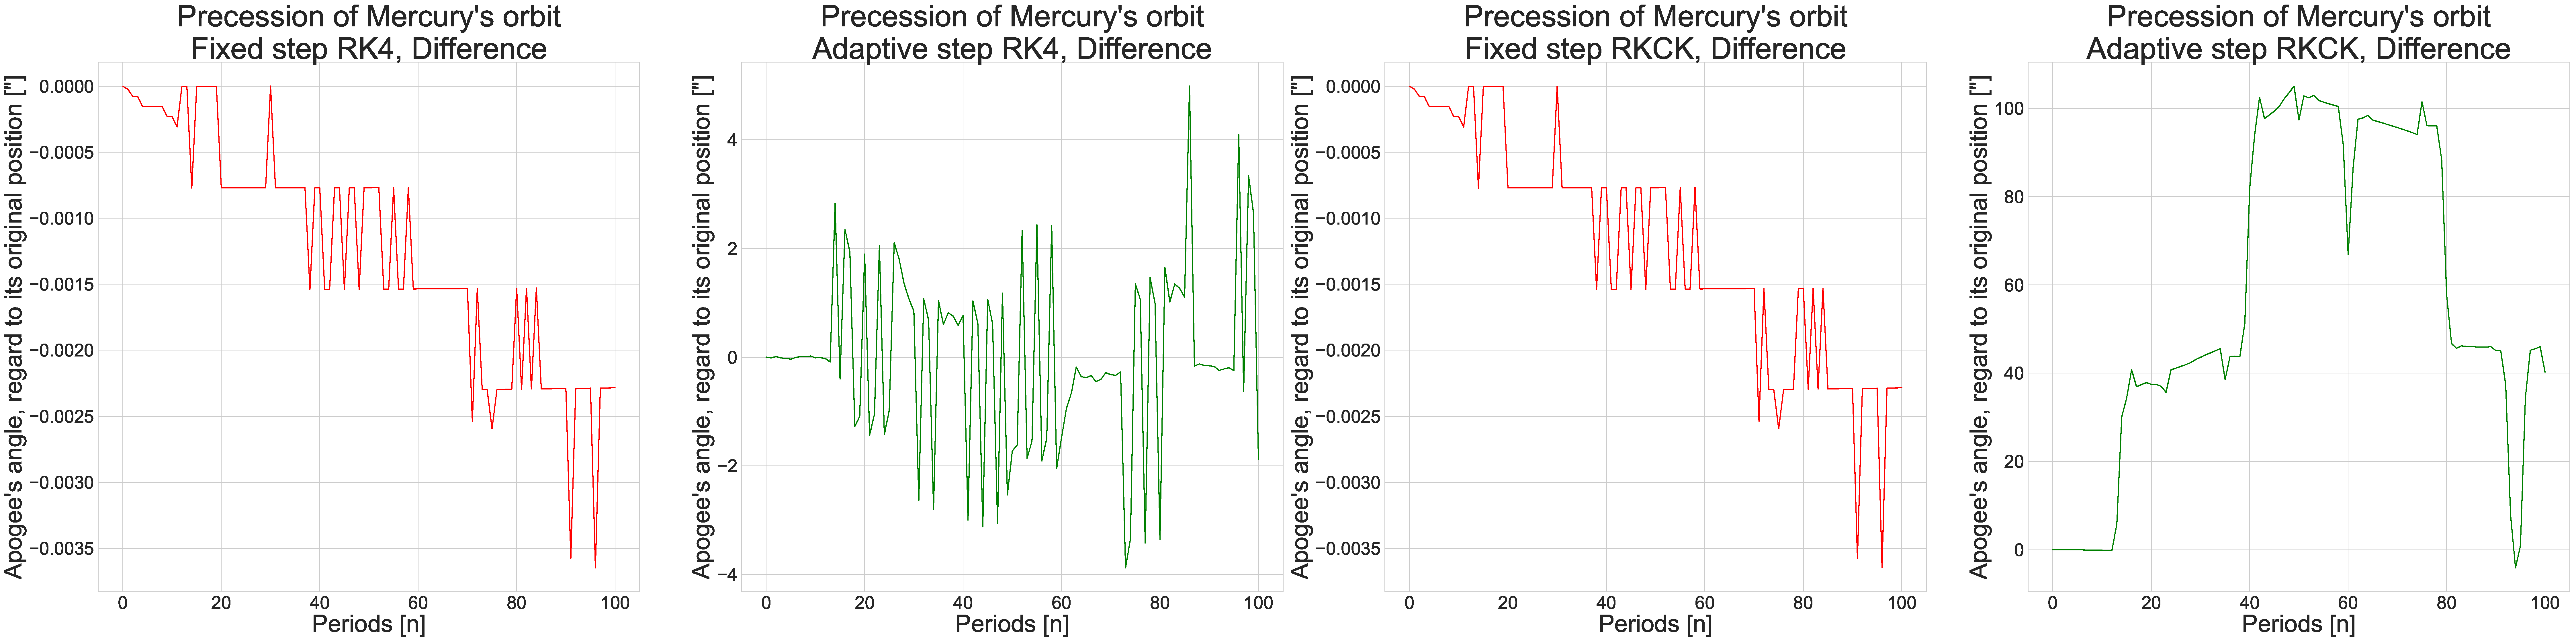
\includegraphics[width=\textwidth]{single_body/Mercury_precession_difference100_dt_1e-04_acc_1e-12.pdf}}
\captionof{figure}{A relativisztikus és a kepleri dinamika különbsége\\Lépésköz nagysága $0.0001 = 10^{-4}$ év}\label{fig:6}

\newpage

\subsection*{A.1.3\ \ Numerikus stabilitás $dt = 10^{-5}$ év esetén}

{\centering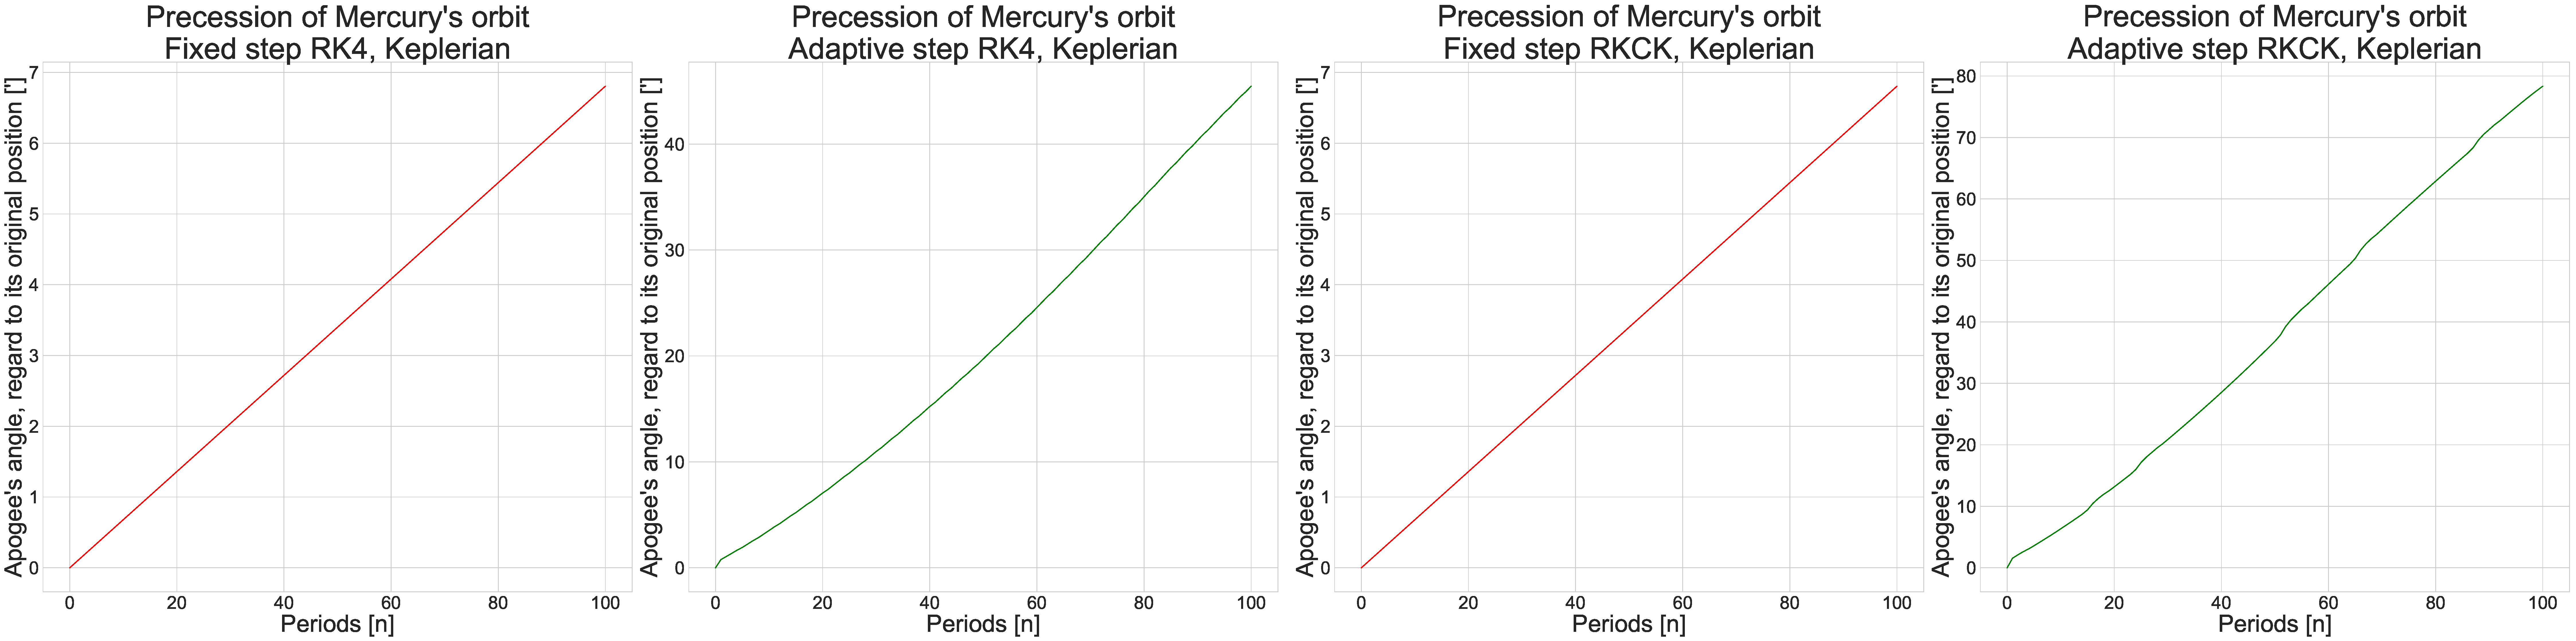
\includegraphics[width=\textwidth]{single_body/Mercury_precession_kepler_dt_1e-05_acc_1e-12.pdf}}
\captionof{figure}{Kepleri dinamika\\Lépésköz nagysága $0.00001 = 10^{-5}$ év}\label{fig:7}
\hfill \break \break
{\centering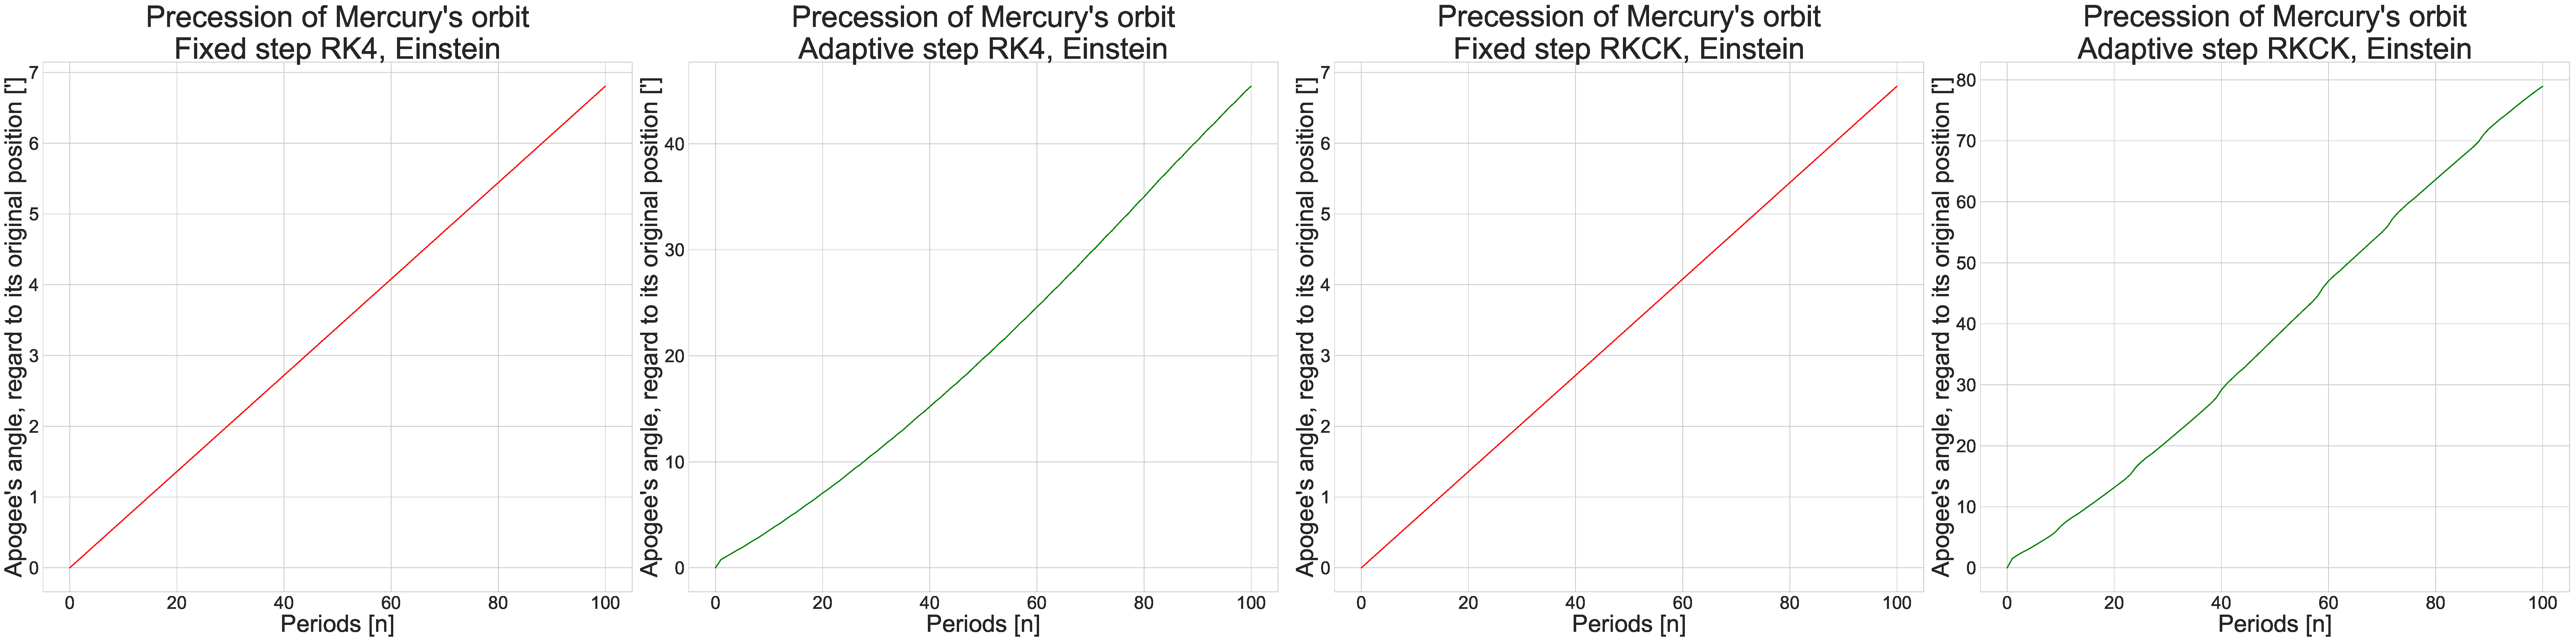
\includegraphics[width=\textwidth]{single_body/Mercury_precession_relat_dt_1e-05_acc_1e-12.pdf}}
\captionof{figure}{Relativisztikus dinamika\\Lépésköz nagysága $0.00001 = 10^{-5}$ év}\label{fig:8}
\hfill \break \break
{\centering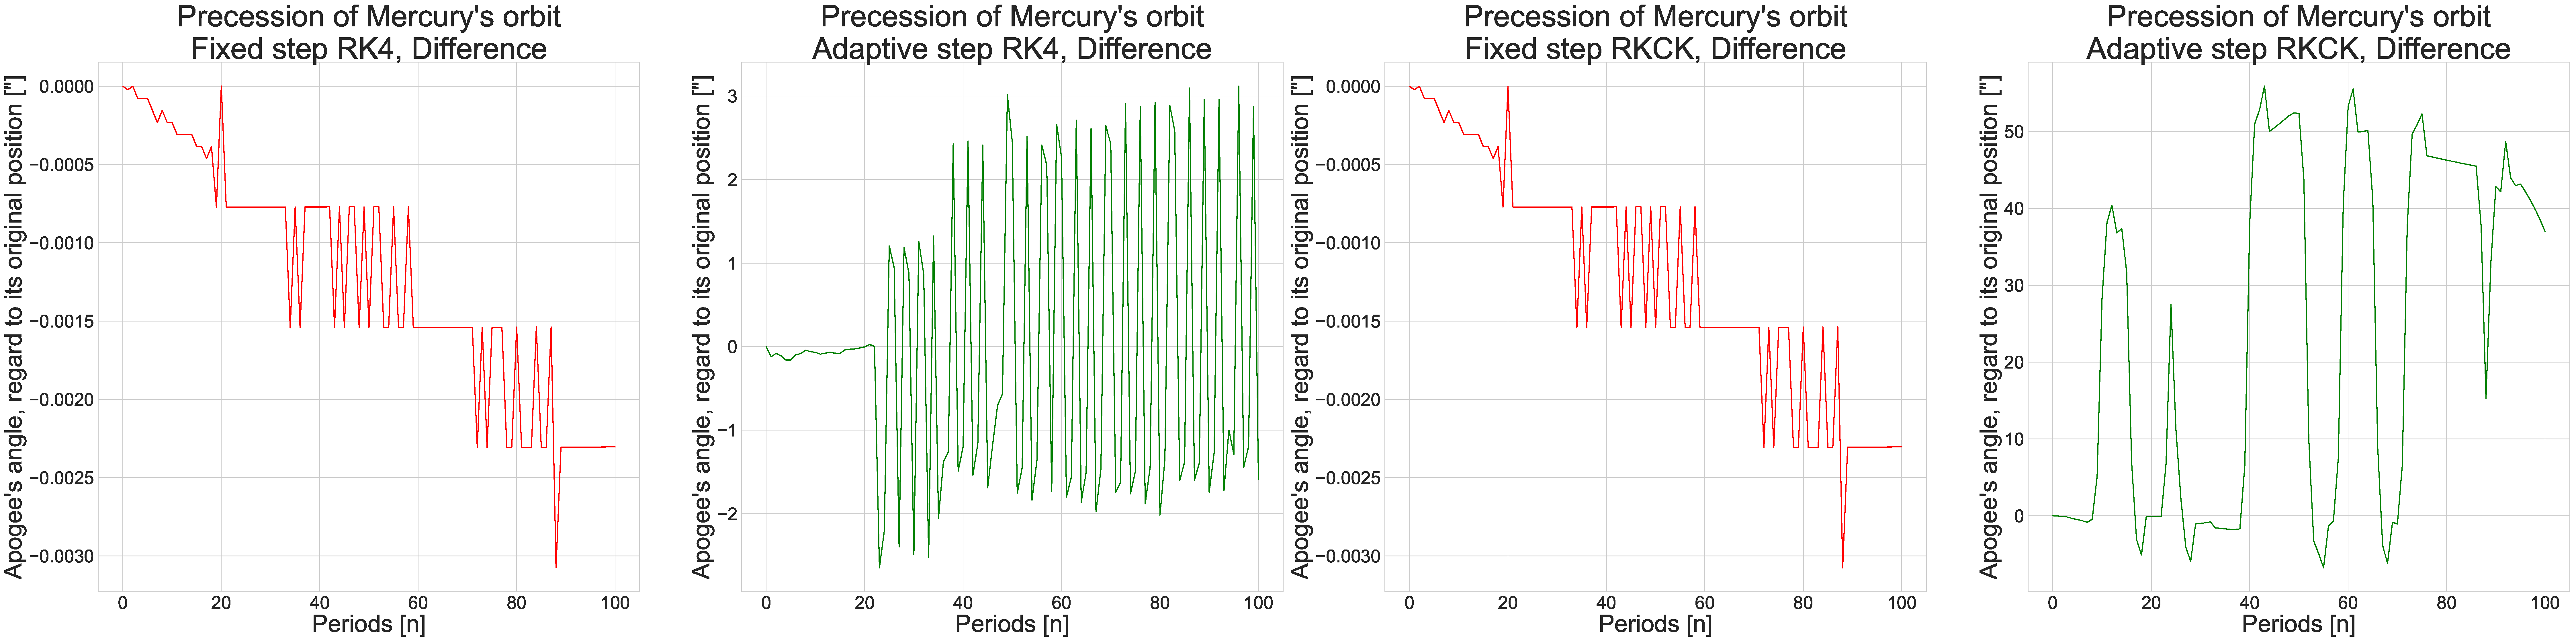
\includegraphics[width=\textwidth]{single_body/Mercury_precession_difference100_dt_1e-05_acc_1e-12.pdf}}
\captionof{figure}{A relativisztikus és a kepleri dinamika különbsége\\Lépésköz nagysága $0.00001 = 10^{-5}$ év}\label{fig:9}

\newpage

\subsection*{A.2.1\ \ Az adaptív lépéshosszak változása klasszikus mozgásegyenletek esetén}

{\centering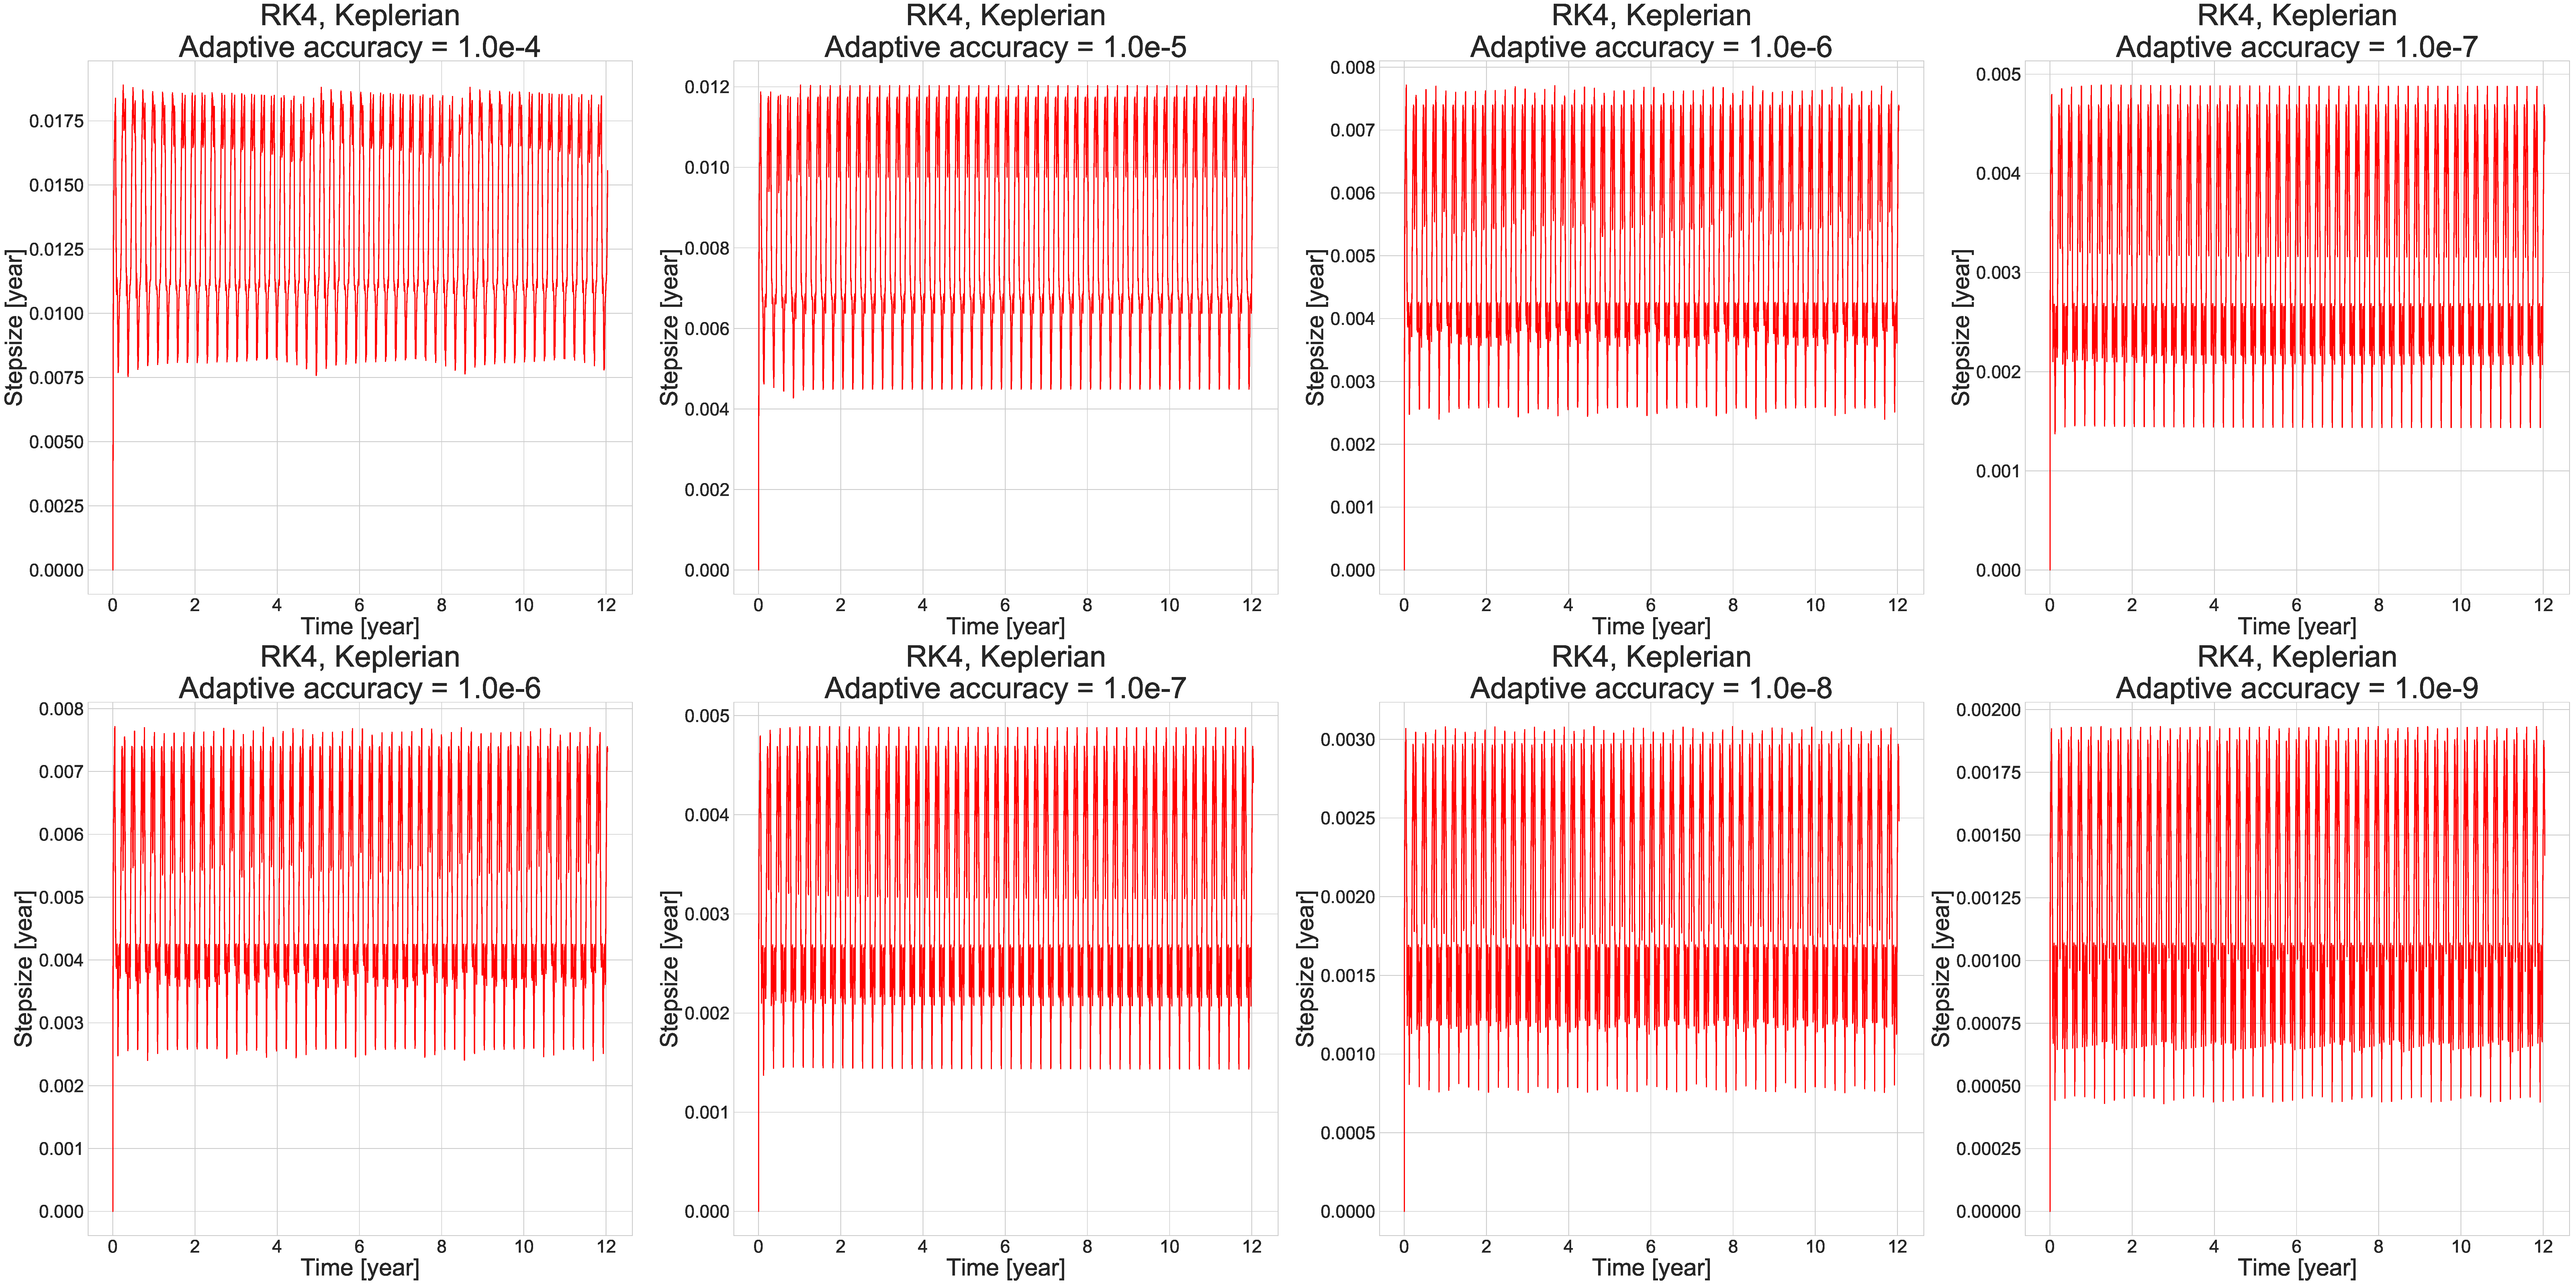
\includegraphics[width=\textwidth]{images/single_body/Mercury_adaptive_accuracy_kepler_runge.pdf}}
\captionof{figure}{Kepleri dinamika\\RK4 módszer; Adaptív lépéshosszak változása az időben}\label{fig:10}
\hfill \break \break
{\centering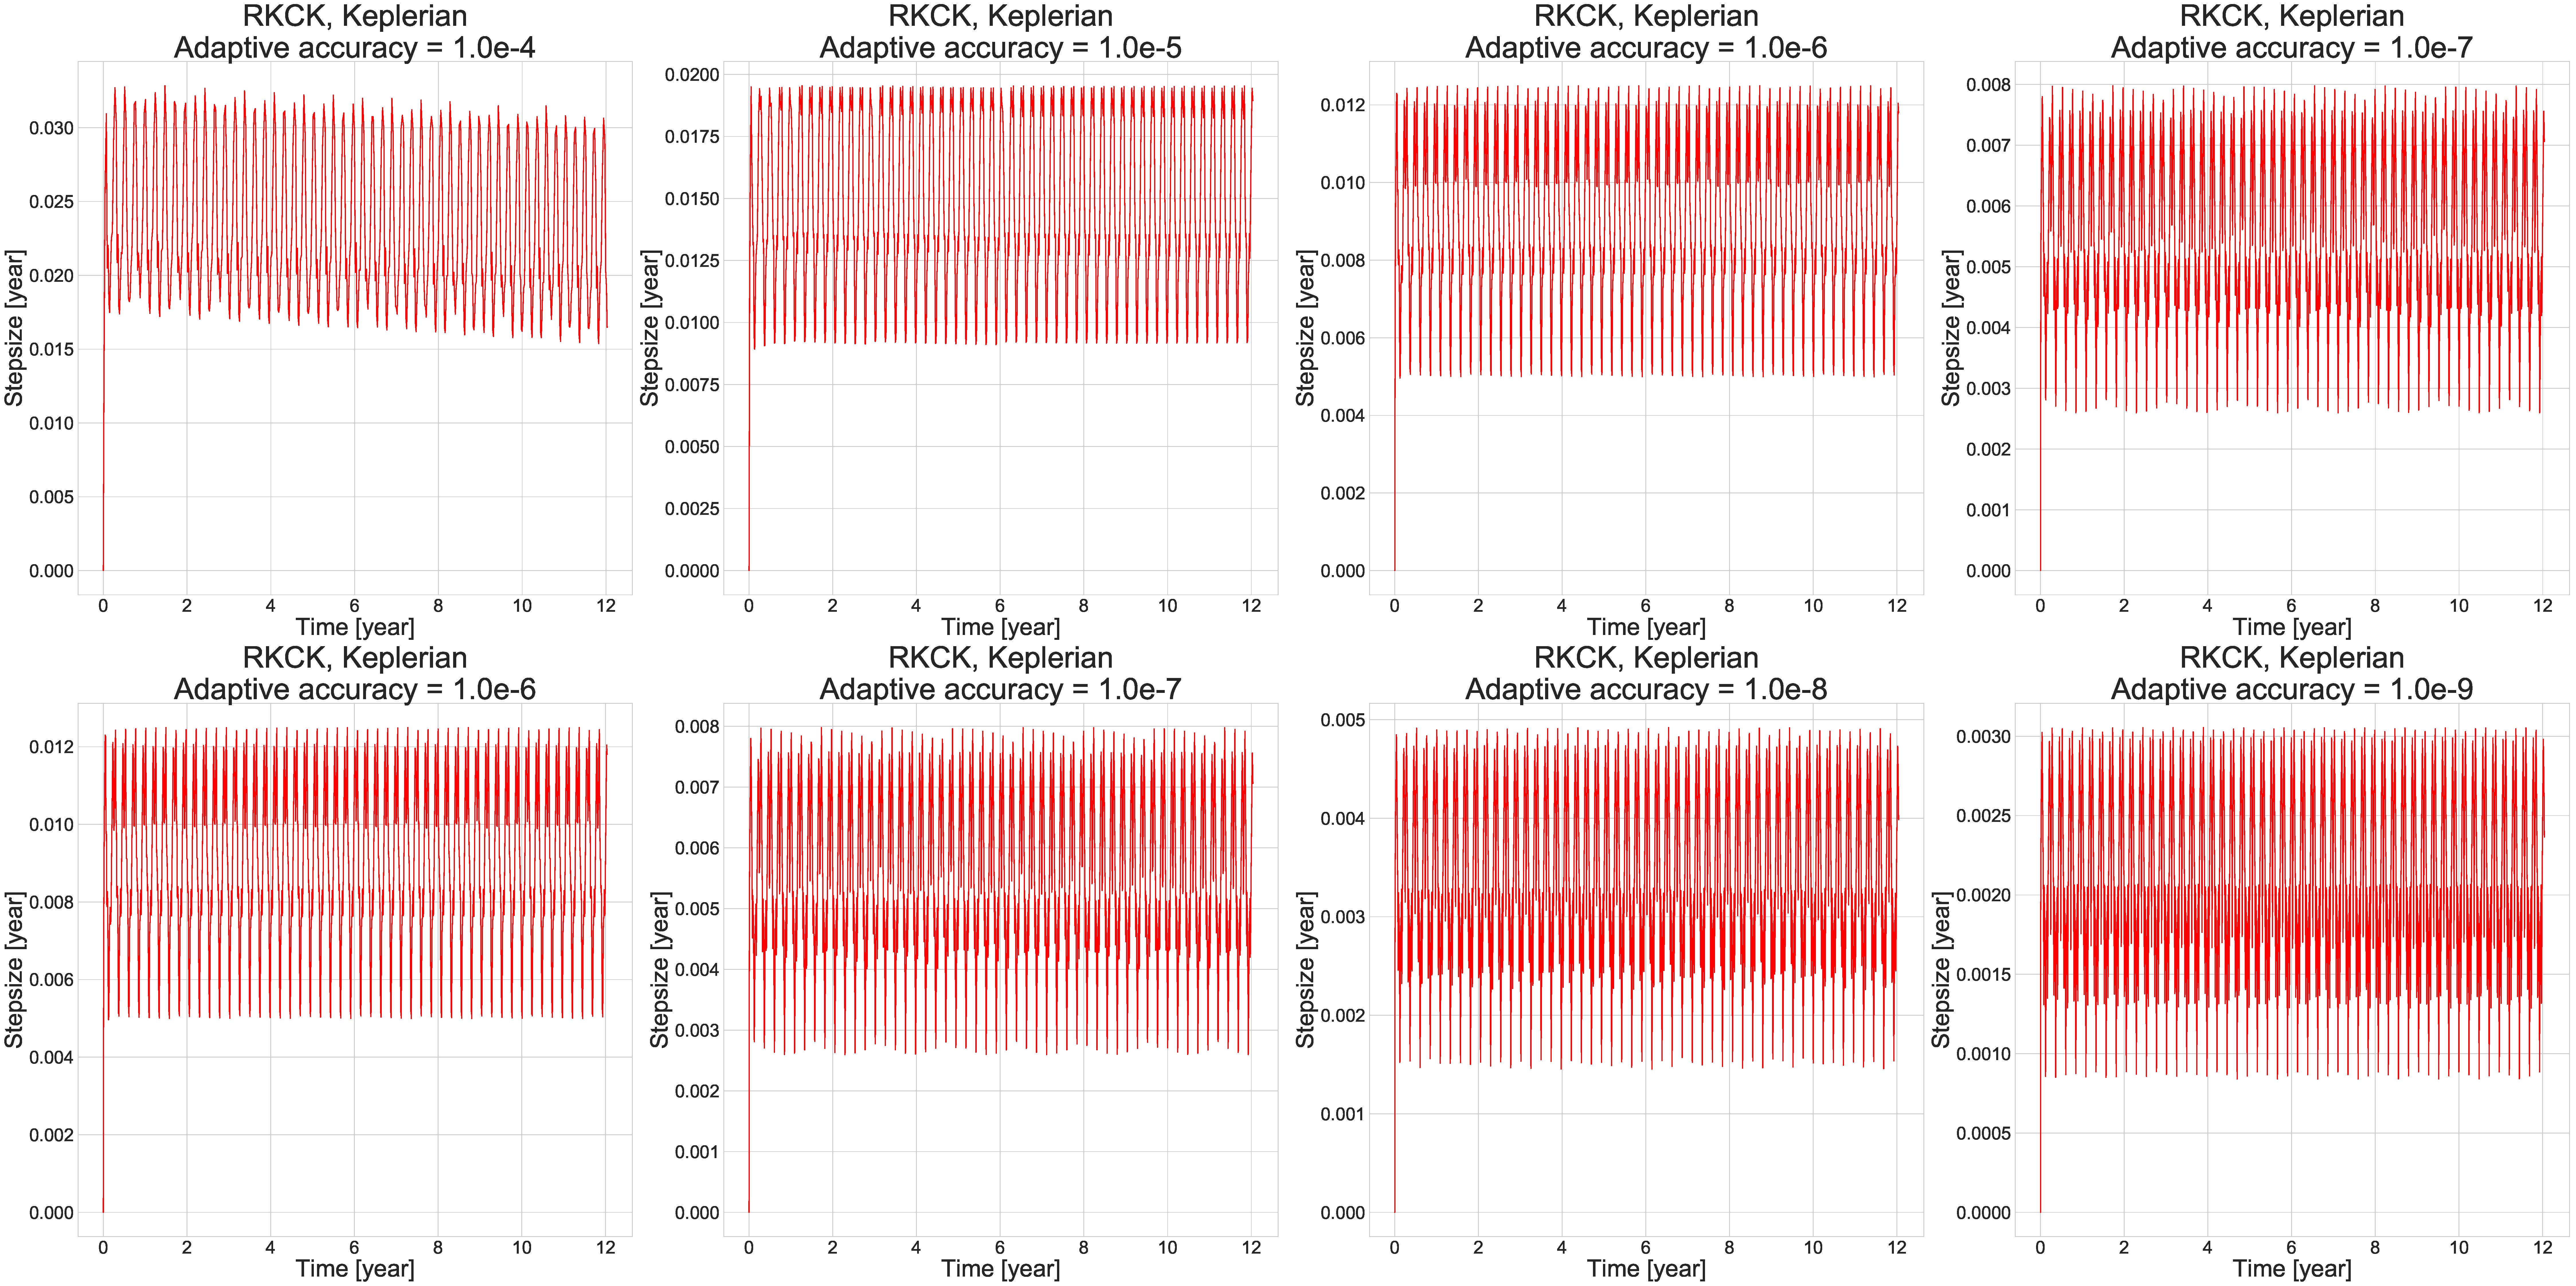
\includegraphics[width=\textwidth]{images/single_body/Mercury_adaptive_accuracy_kepler_rkck.pdf}}
\captionof{figure}{Kepleri dinamika\\RKCK módszer; Adaptív lépéshosszak változása az időben}\label{fig:11}

\newpage

\subsection*{A.2.2\ \ Az adaptív lépéshosszak változása relativisztikus mozgásegyenletek esetén}

{\centering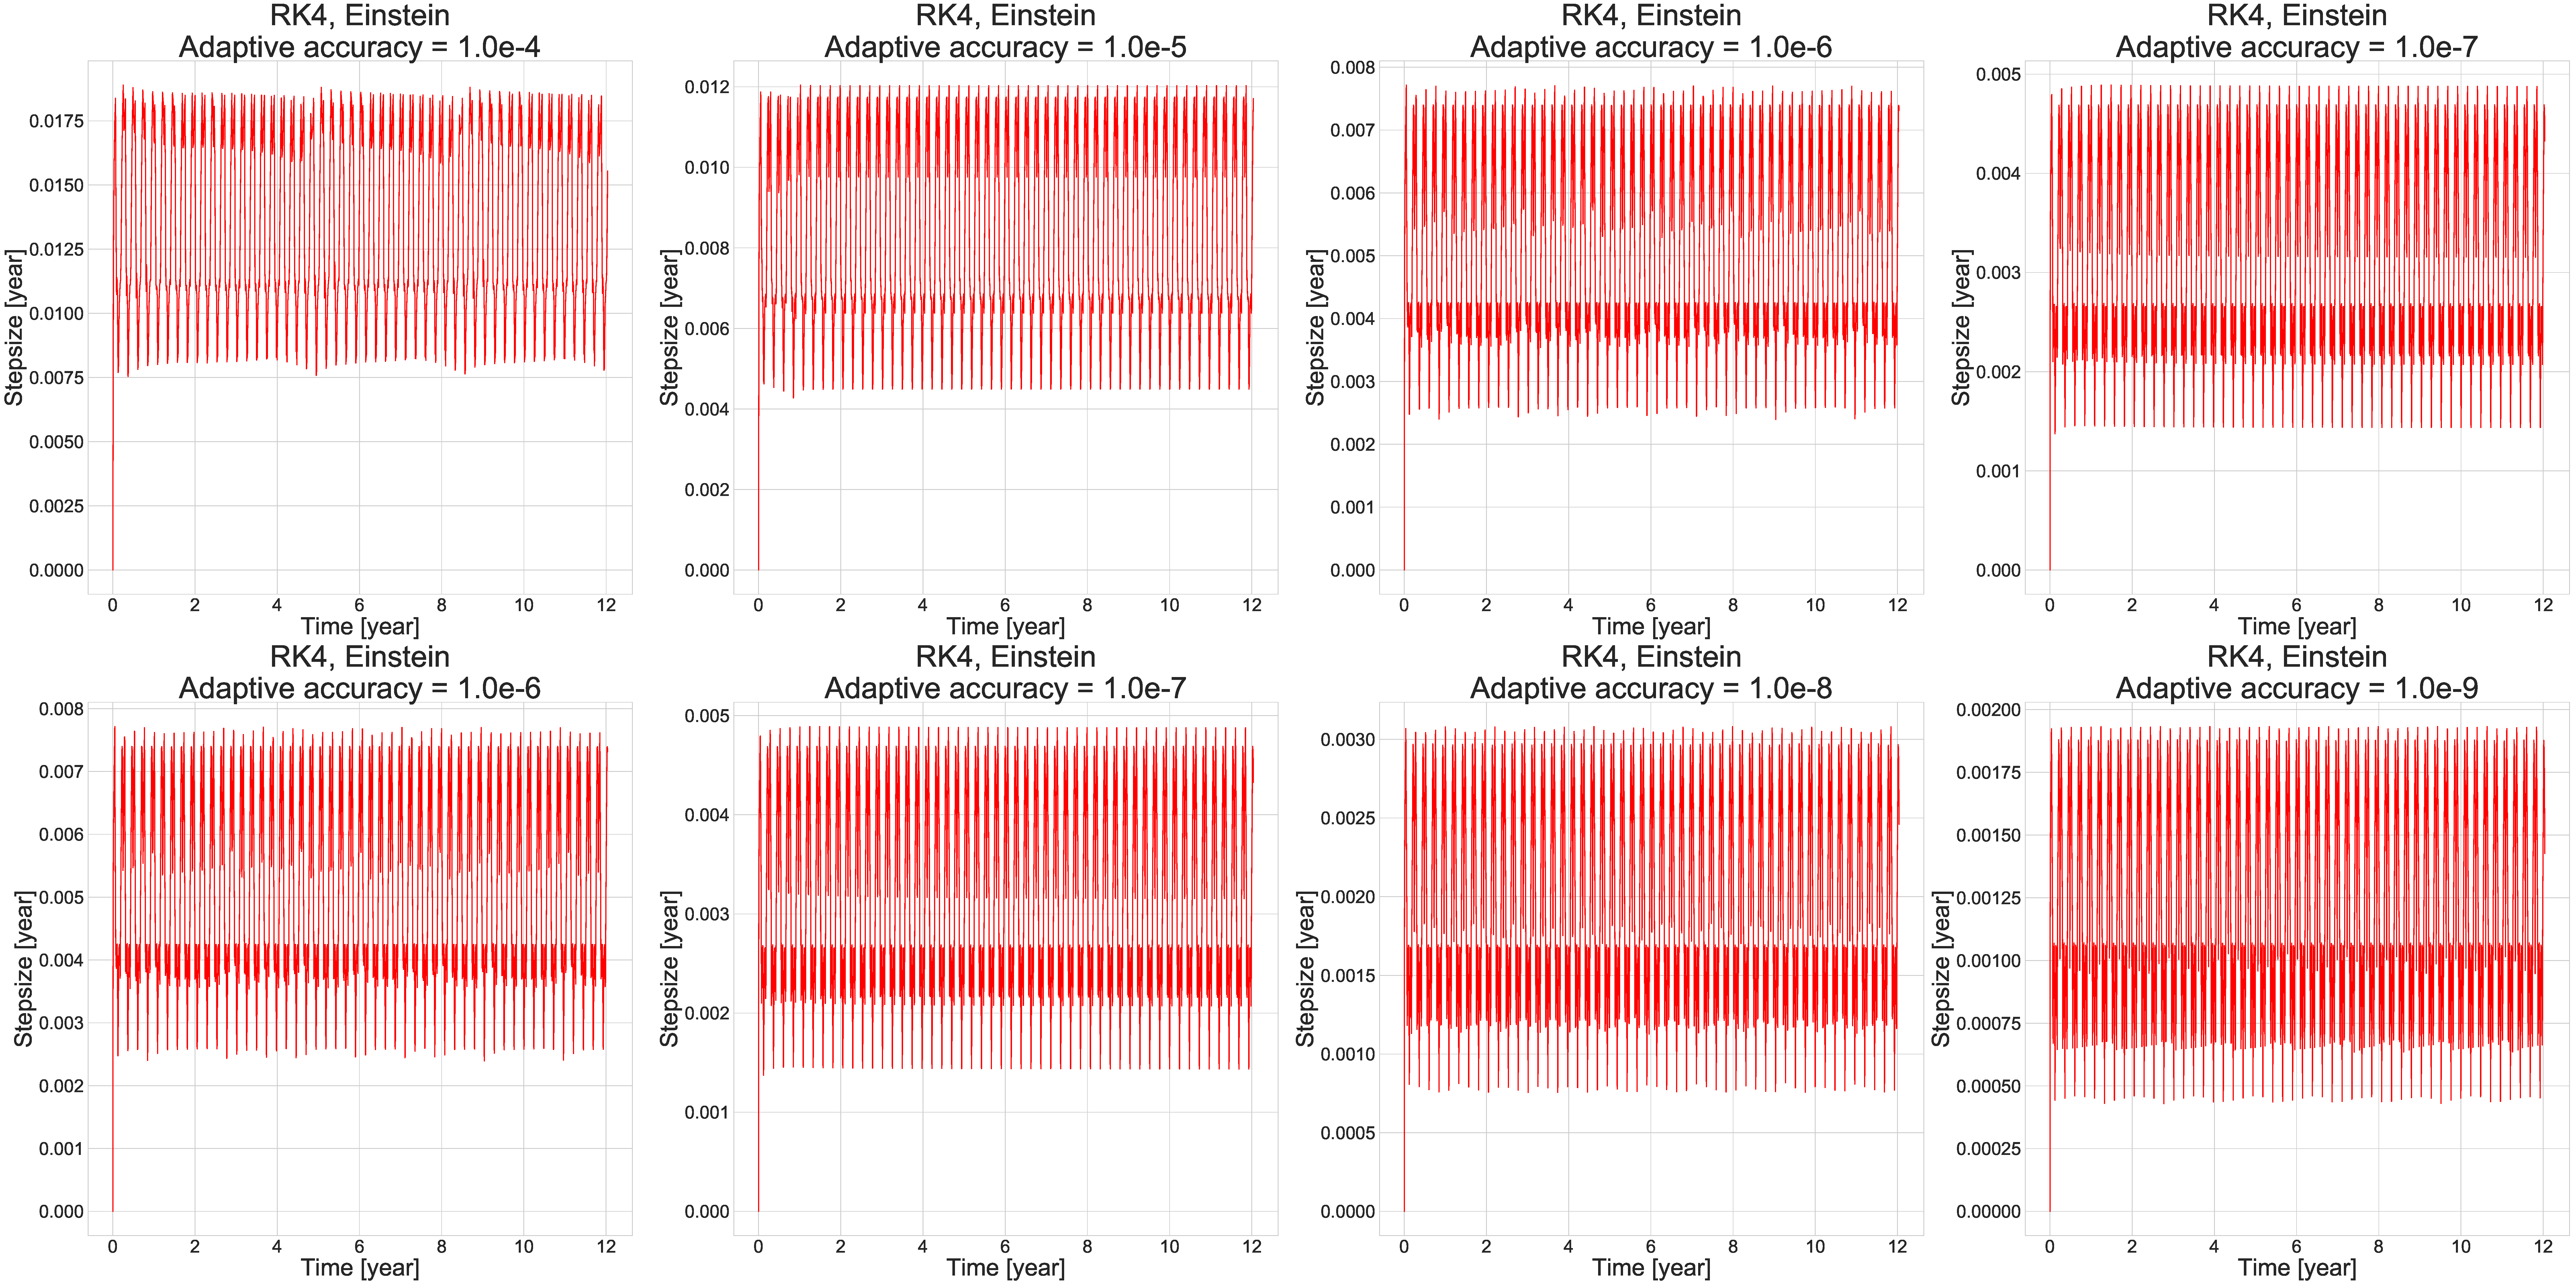
\includegraphics[width=\textwidth]{images/single_body/Mercury_adaptive_accuracy_einstein_runge.pdf}}
\captionof{figure}{Relativisztikus dinamika\\RK4 módszer; Adaptív lépéshosszak változása az időben}\label{fig:12}
\hfill \break \break
{\centering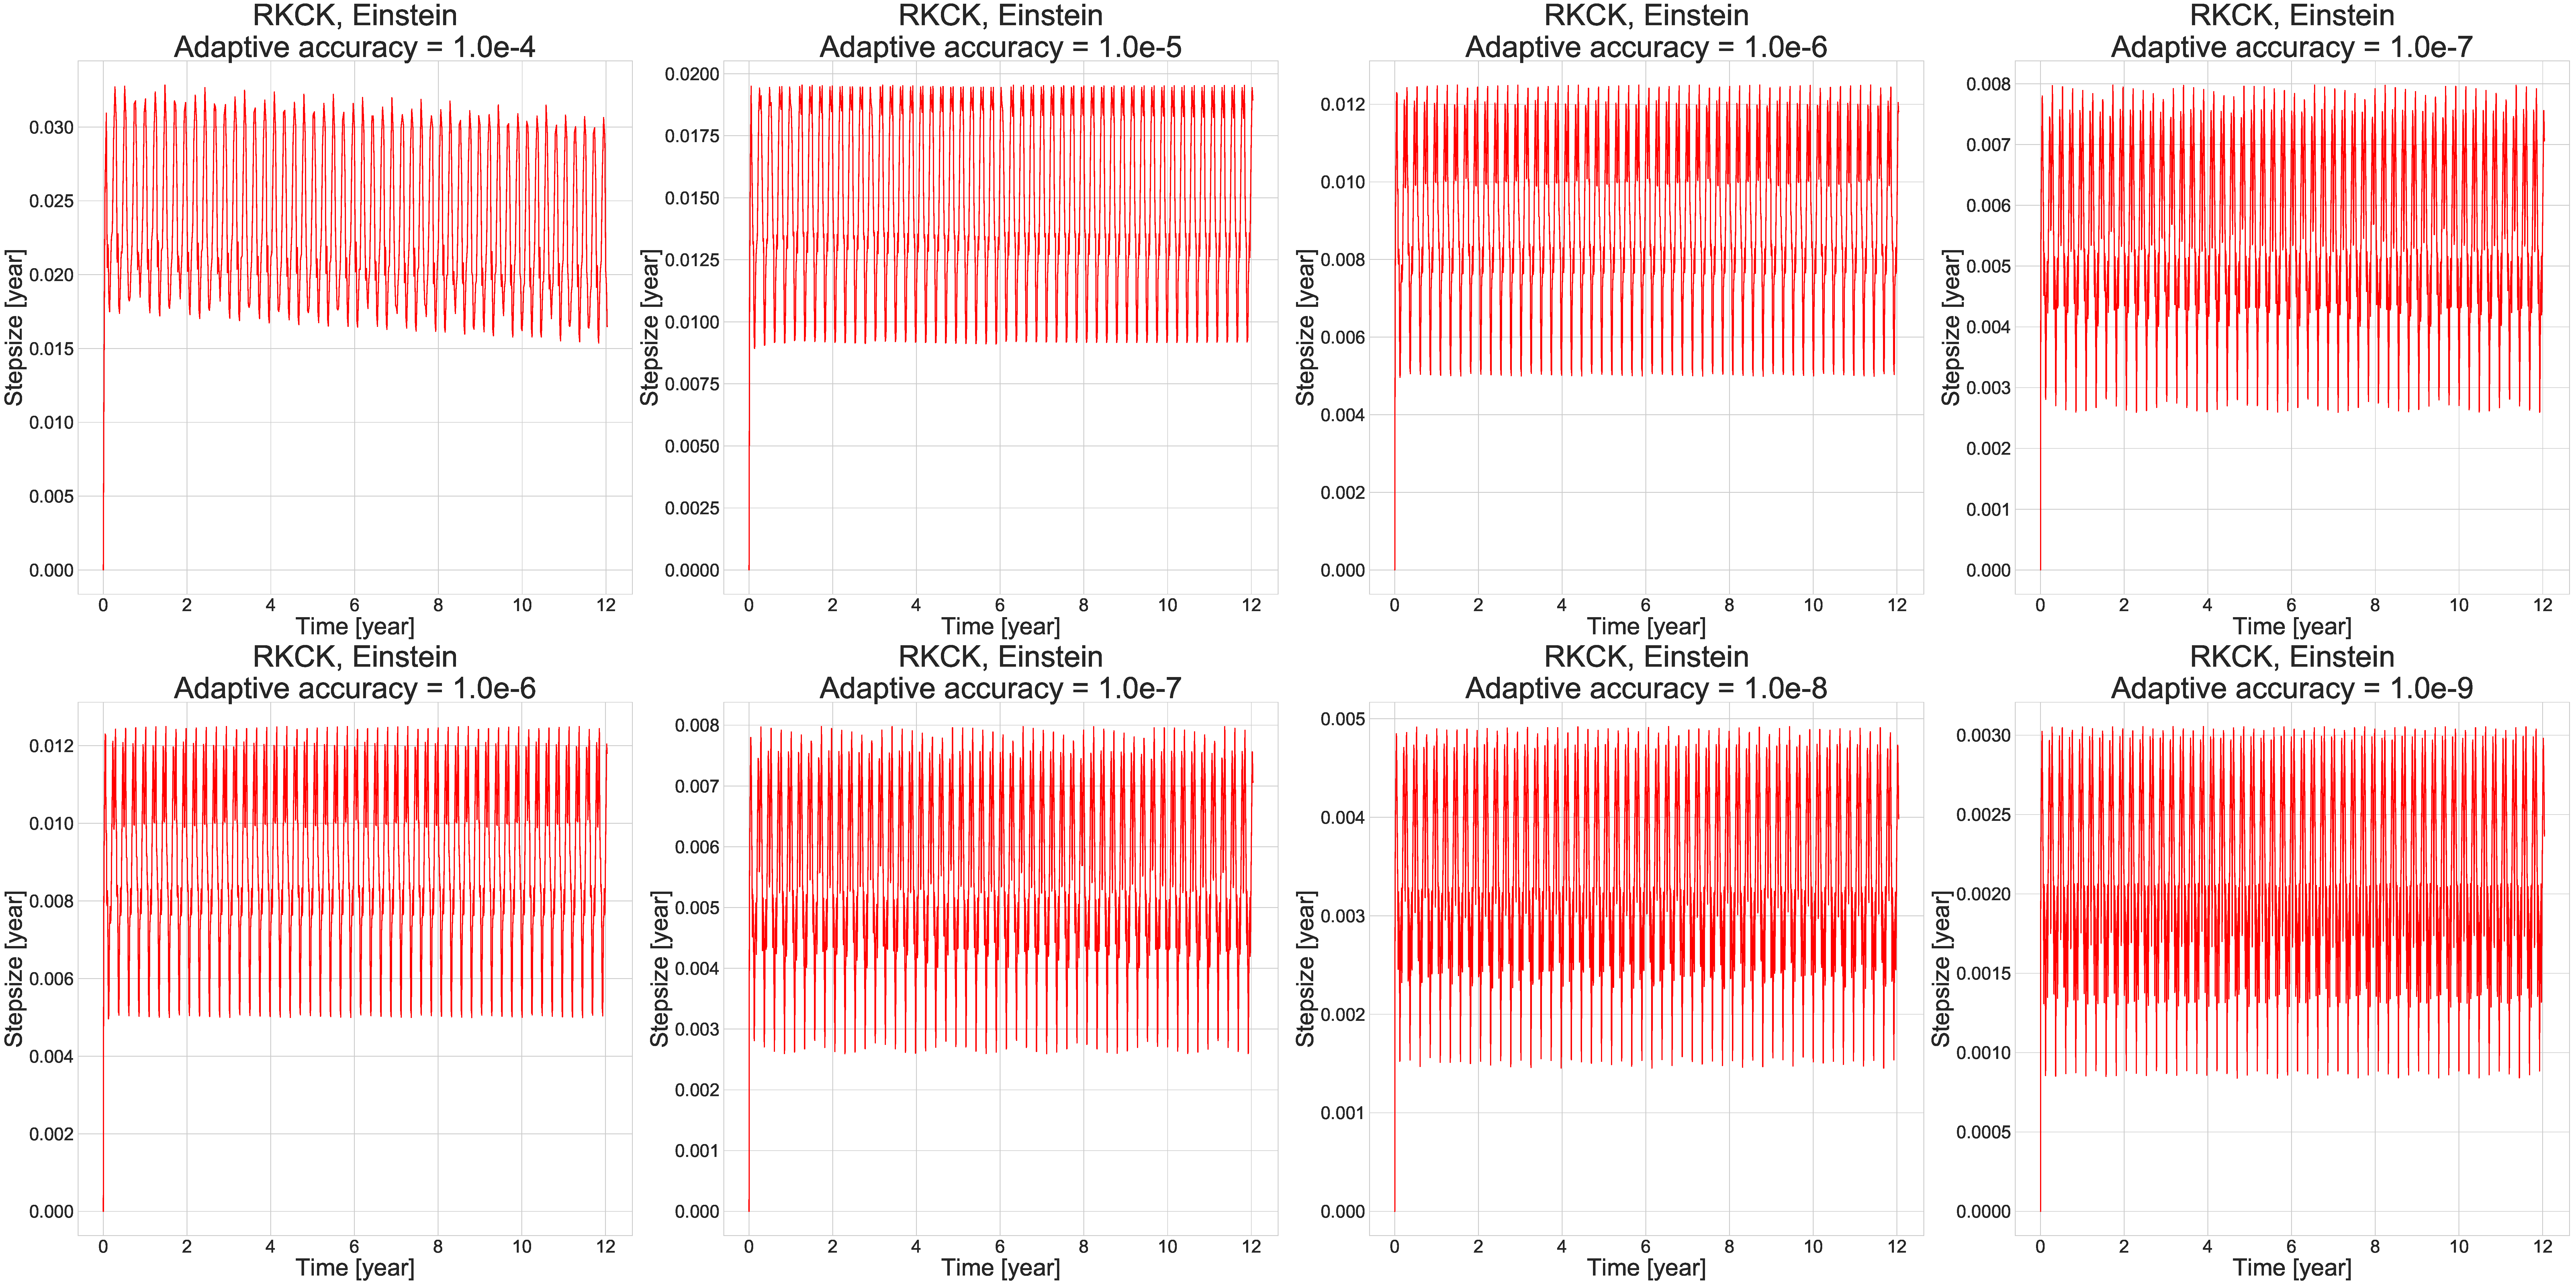
\includegraphics[width=\textwidth]{images/single_body/Mercury_adaptive_accuracy_einstein_rkck.pdf}}
\captionof{figure}{Relativisztikus dinamika\\RKCK módszer; Adaptív lépéshosszak változása az időben}\label{fig:13}

\newpage

{\centering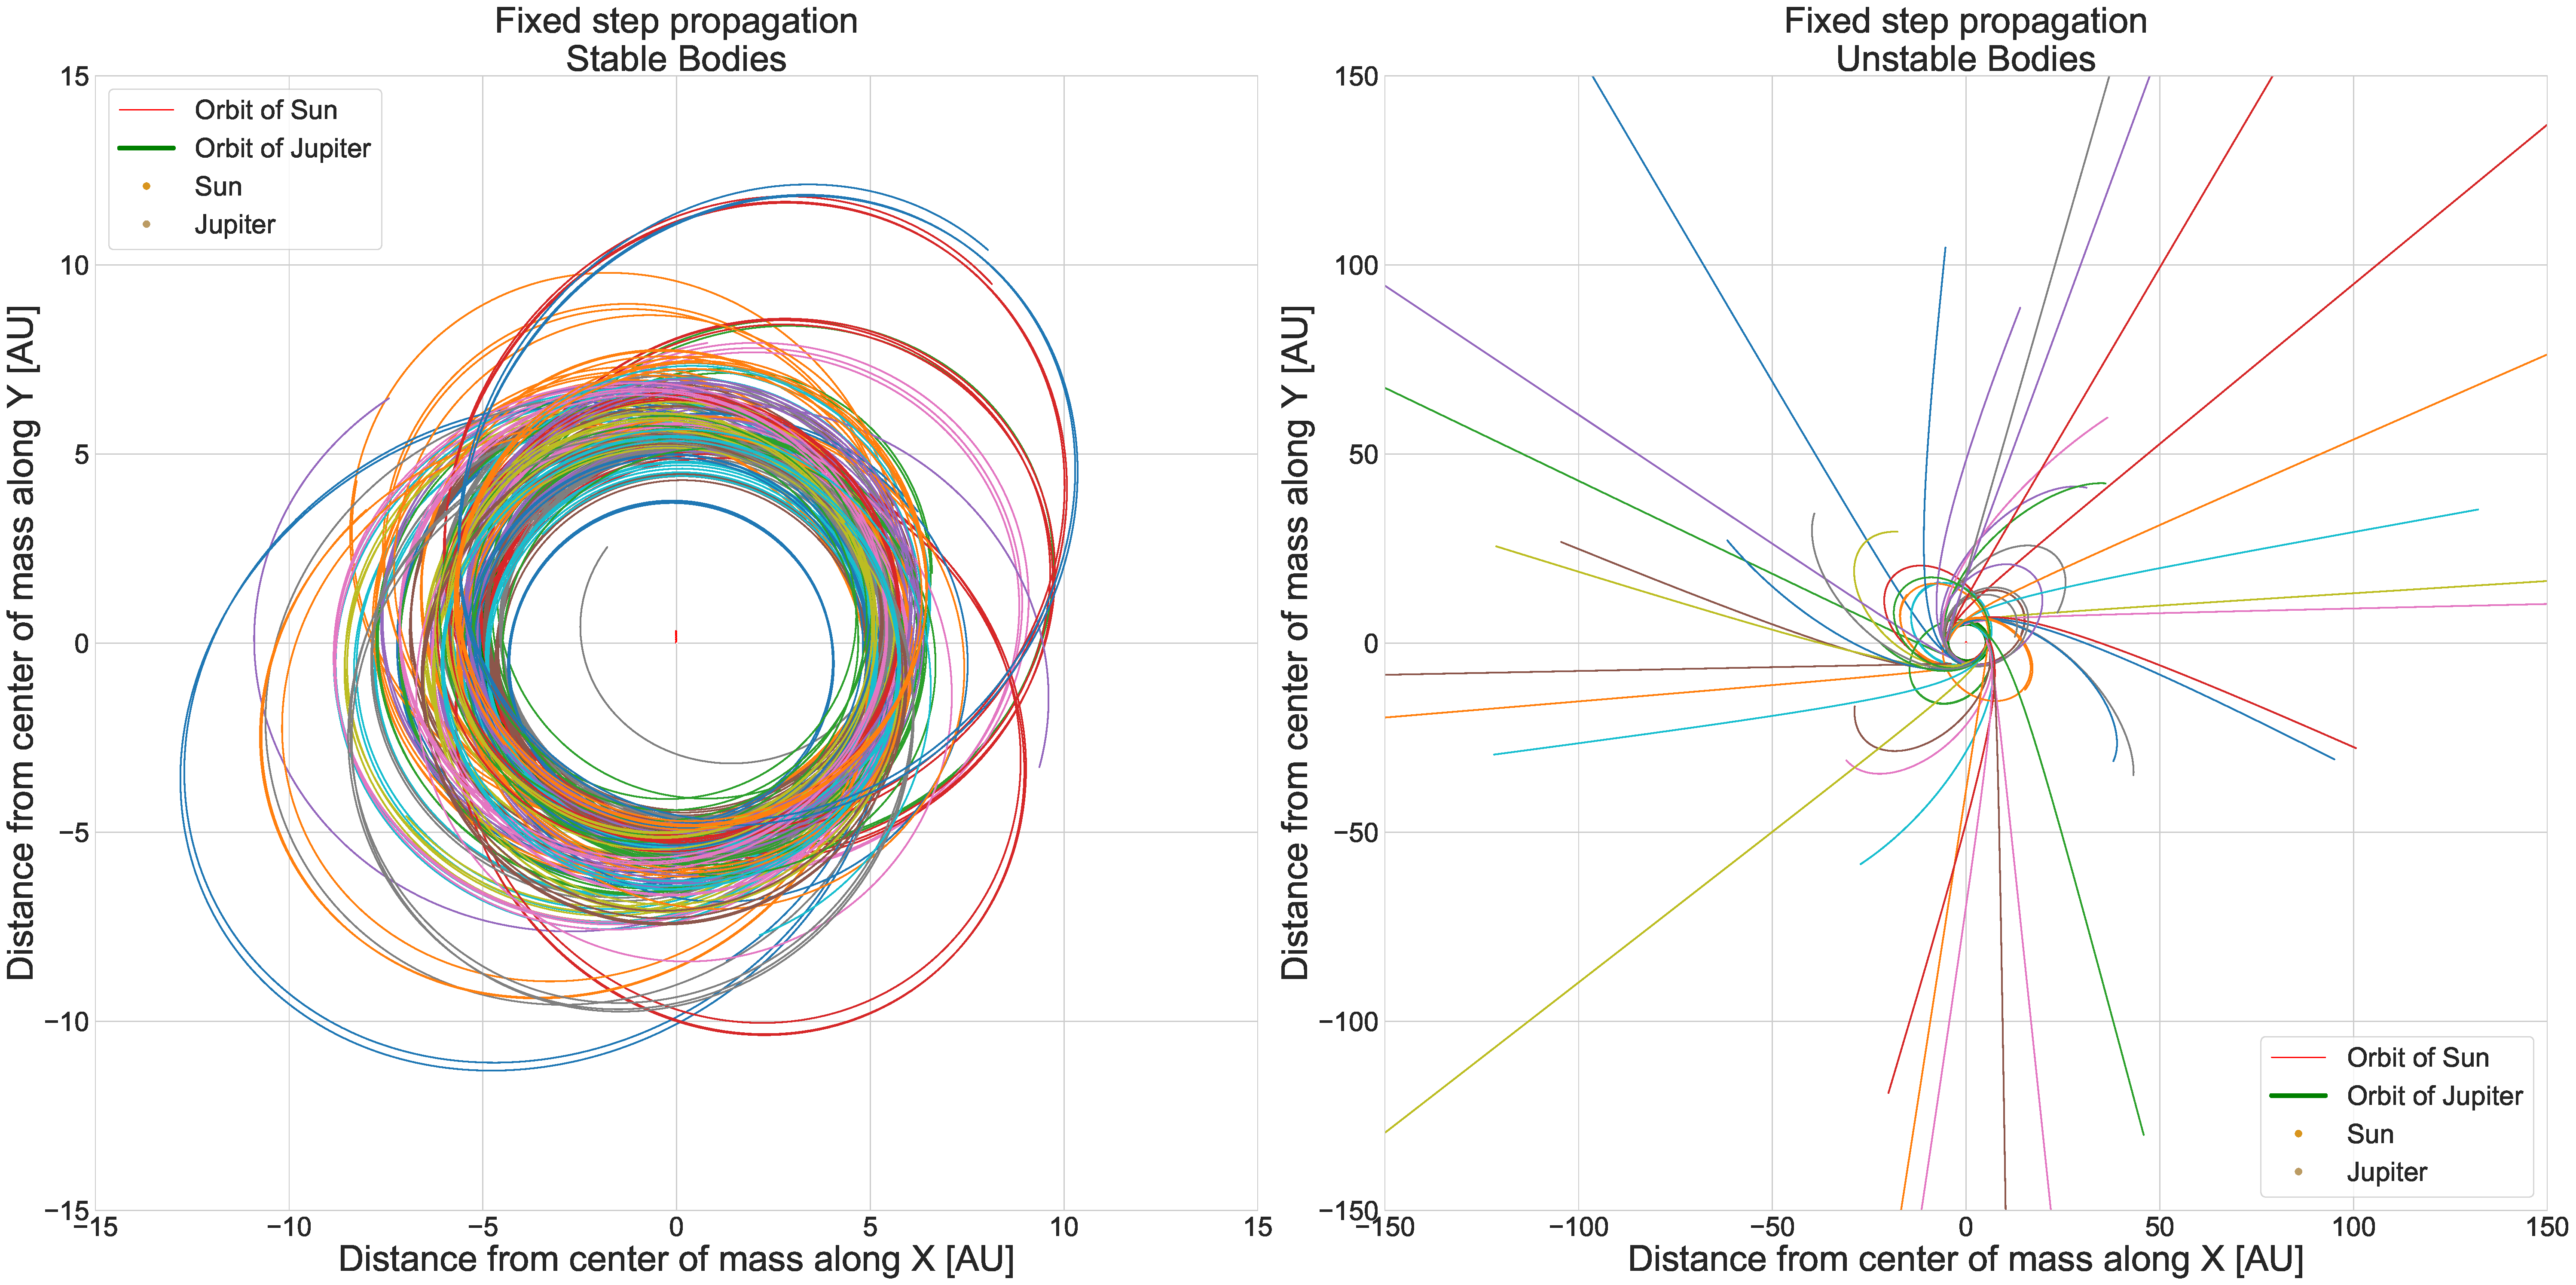
\includegraphics[width=\textwidth]{images/Jupiter_around_Sun_fixed.pdf}}
\captionof{figure}{A Jupiter-Nap rendszer mozgása 40, véletlenszerűen a Jupiter pályája köré szórt testtel szimulálva}\label{fig:14}